\chapter{相关工作}

\section{概率主题模型}
概率主题模型 \cite{griffiths2004finding, Blei:2003, hofmann1999probabilistic, hofmann2001unsupervised} 的基本思想是:文档可以被看成主题的分布,而主题可以看成是词的概率分布。主题模型是关于文档的生成模型,文档的生成过程包含以下几个步骤:首先为文档确定一个基于主题的概率分布,对于文档中的每个词,随机的从主题概率分布中选择一个主题,然后从与该主题对应的词的分布中随机选择一个词。如图 \ref{fig:topic-distribution-sample} 所示,主题可以用概率最大的前几个词来表示。
% BEGIN == 主题分布 例子
\begin{figure}[htb]
    \centering%
    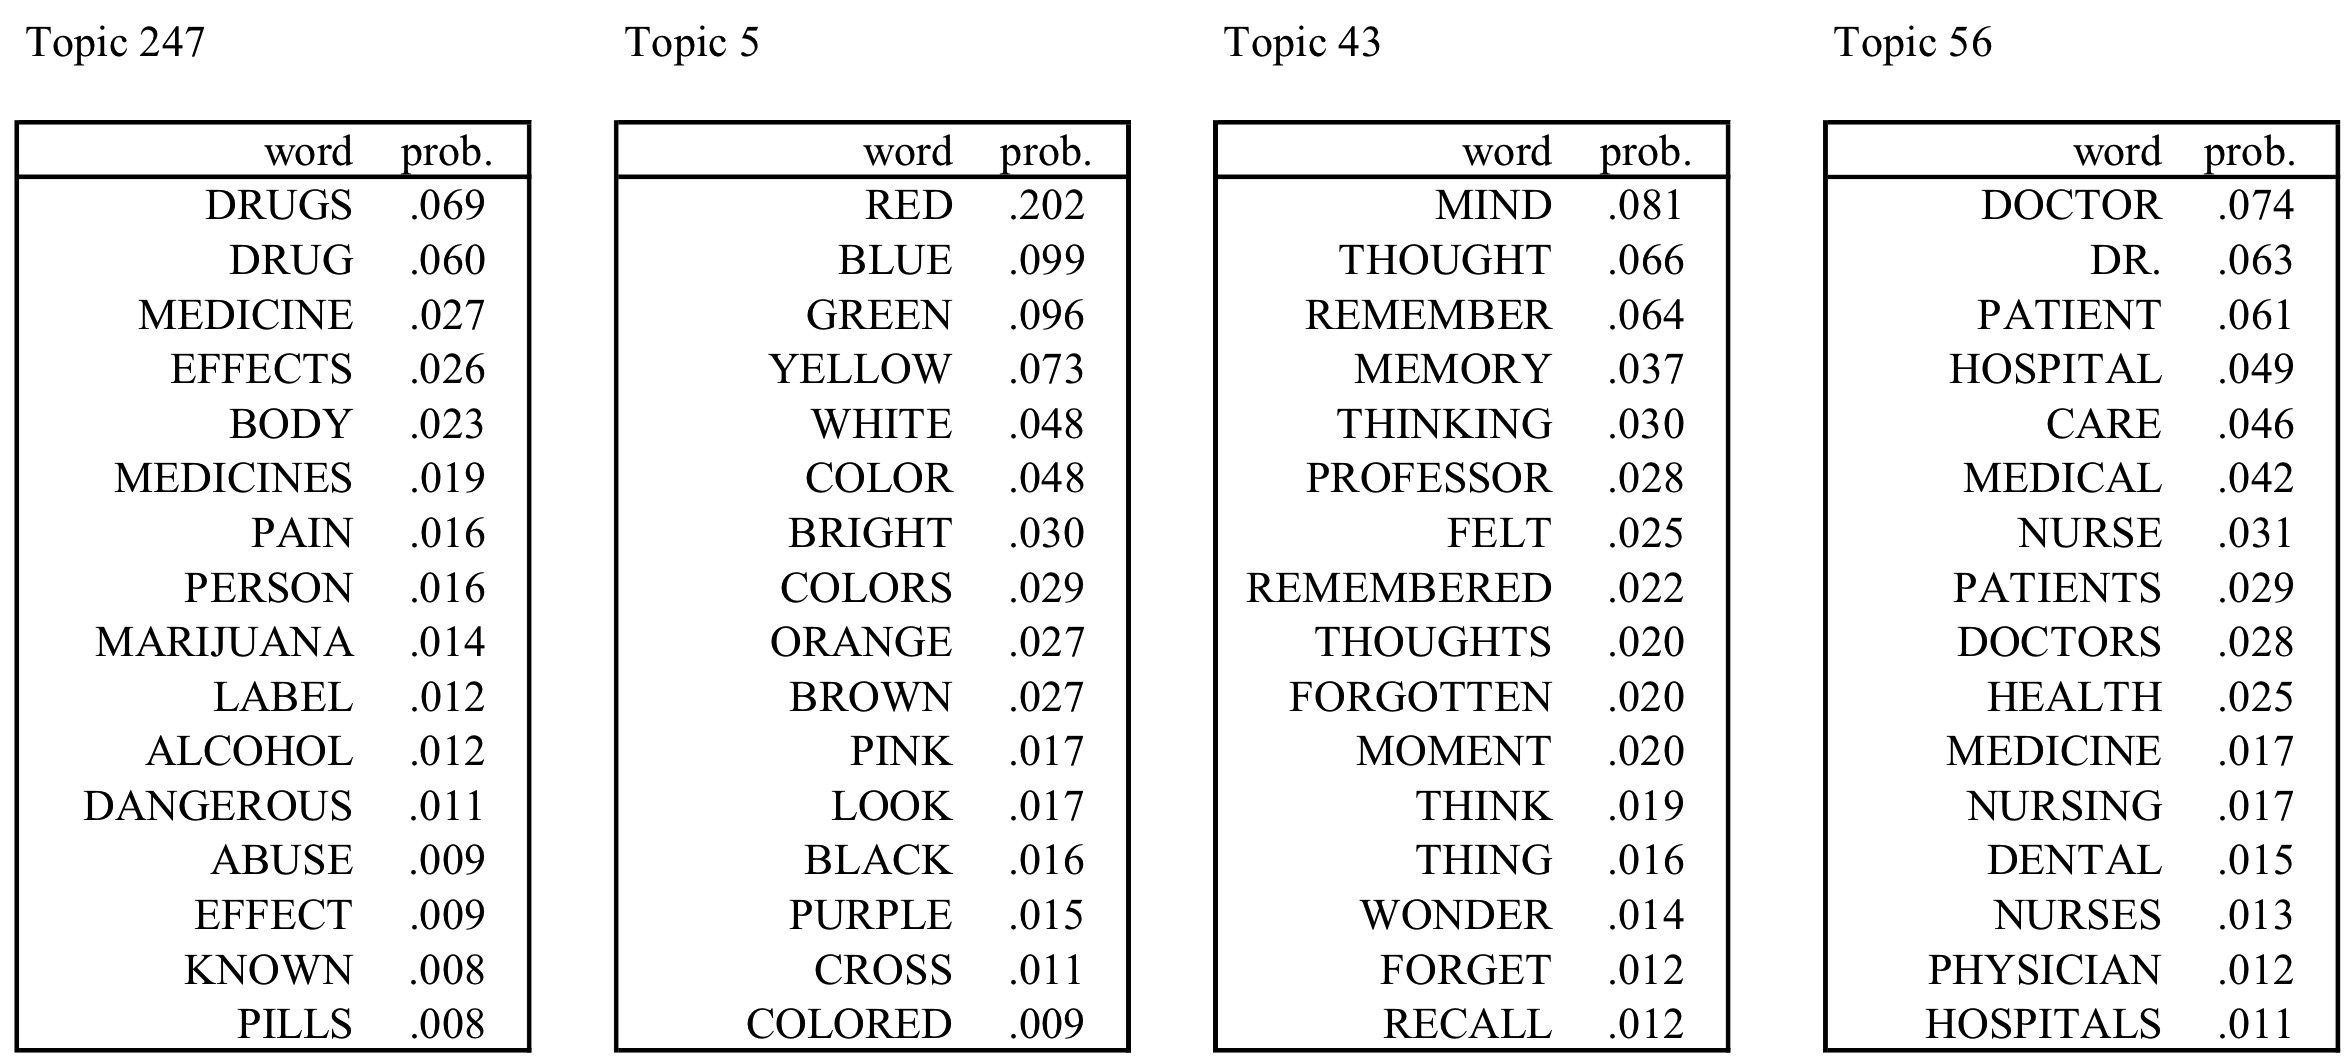
\includegraphics[width=\textwidth]{topic-distribution-sample}
    \caption{主题~词的概率分布例子}
    \label{fig:topic-distribution-sample}
\end{figure}
% END == 主题分布 例子

\subsection{LDA}
\label{intro-lda}
LDA\cite{Blei:2003}模型假定语料库 $D$ 中文档 $d$ 的生成过程如下:\\
% BEGIN == 自适应聚类算法 伪代码
\begin{algorithm}[!htb]
  采样 $N \sim Poisson(\xi)$\;
  采样 $\phi_d \sim Dir(\alpha)$\;
  \For{文档 $d_n$ 中的 $N$ 个单词}{
        采样一个主题标签 $z \sim Multi(\phi_d)$\;
        确定单词 $w \sim Multi(\theta_z)$\;
      }
  \caption{LDA 文档生成过程}
  \label{lda-generative-process}
\end{algorithm}
% END == 自适应聚类算法 伪代码

其中$\theta_{(\cdot)} \sim Dir(\beta)$。在LDA模型中,有两组先验,一个是文档~主题的先验,来自于一个对称的$Dir(\alpha)$;另一个是主题~词汇的先验,来自于一个对称的$Dir(\beta)$。LDA图模型如图 \ref{fig:lda-graph-model}所示。
\begin{figure}[htb]
    \centering%
    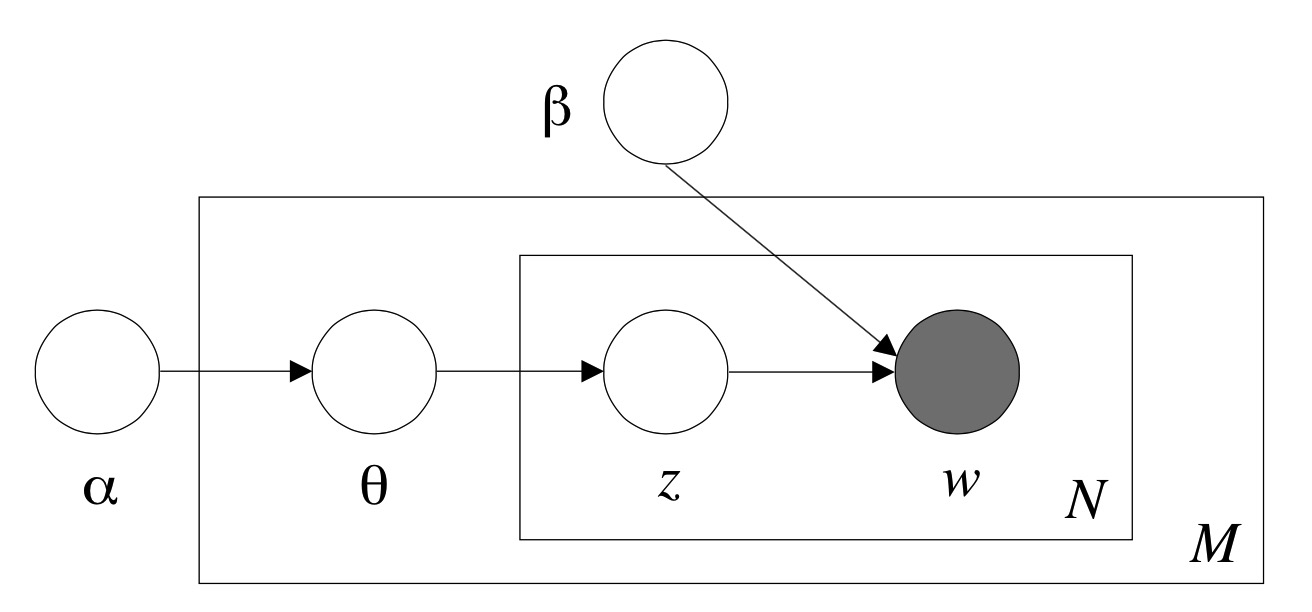
\includegraphics[width=0.6\textwidth]{lda-graph-model}
    \caption{LDA 图模型。}
    \label{fig:lda-graph-model}
\end{figure}

要理解LDA,我们需要明白以下的一些知识:
\begin{itemize}
\item 贝叶斯层级模型。LDA是完全的贝叶斯模型,它把$\phi_{(\cdot)}$和$\theta_{(\cdot)}$都看做是随机变量,分别由超参数$\alpha$和$\beta$控制。
\item 隐变量模型。LDA本质上一种隐变量模型,LDA名字中的"Latent"正是表达这个意思,隐变量模型的意思是指引入一些中间变量,而这些变量在数据中并无体现,引入中间隐含变量的目的是为使得模型的描述和推导更加明了。
\item 可交换性。可交换性是指,给定随机变量序列${z_1, z_2, ... , z_n}$,对于该序列的任何一个置换$\pi$,都能使得联合分布 $p(z_1, ..., z_n)=p(z_{\pi(1)}, ..., z_{\pi(n)})$。LDA中假设词是由主题产生的,并且这些主题在该文档中是可交换的。
\end{itemize}

\subsubsection*{参数学习}
虽然LDA模型相对而言并不复杂,但是具体的参数推导却几乎是不可能的,其中一个方法是采用近似推导算法,如吉布斯采样\cite{griffiths2004finding}。\par
吉布斯采样是马尔可夫链蒙特卡罗模拟(Markov Chain Monte Carlo, MCMC)\cite{mackay2003information}的一个特例,并且比较适合在高维模型中进行近似推导。MCMC方法通过利用了马尔可夫链的平稳分布特性来仿真高维度的概率分布$p(\vec{x})$。也就是说,当马尔可夫链达到稳定状态后,每一次状态转移可以进行一次采样\cite{Walsh:2004}。吉布斯采样每次采样获得$x_i$的一个维度,通过迭代可以获得$\vec{x}$。参数推导的目标是$p(\vec{z}|\vec{w})$,该条件分布正比于联合分布(见公式 (\ref{eq:union-dist}))。其中$z_{m,n}$表示文档$m$中的第$n$个词的主题。
\begin{equation}
\label{eq:union-dist}
p(\vec{z}|\vec{w})=\frac{p(\vec{z}, \vec{w})}{p(\vec{w})} \propto p(\vec{z}, \vec{w}) = p(\vec{z}, \vec{w}|\vec{\alpha},\vec{\beta}) = p(\vec{w}|\vec{z},\vec{\beta})p(\vec{z}|\vec{\alpha})
\end{equation}
由于多项式分布与Dirichlet分布共轭,所以 $\varphi_k$ 和 $\vartheta_m$ 在积分过程中能被抹掉。从联合概率分布中,我们可以派生出词 $i=(m,n)$ 的全条件概率分布$p(z_i=k|\vec{z}_{\neg i},\vec{w})$。当$\vec{z}$的所有维度都推导出来后,我们可以通过Dirichlet分布的期望来计算公式(\ref{eq:varphi})和(\ref{eq:vartheta})(具体细节可以参见\cite{heinrich2005parameter}):
\begin{equation}
\label{eq:varphi}
\varphi_{k,t}=\frac{n_{k}^{t}+\beta_{t}}{\sum_{t=1}^{V}n_{k}^{t} \; +\beta_{t}}
\end{equation} 
\begin{equation}
\label{eq:vartheta}
\vartheta_{m,k}=\frac{n_{m}^{k}+\alpha_k}{\sum_{k=1}^{K}n_{m}^{k} \; +\alpha_k}
\end{equation} 

\subsection{DTM}
\label{intro-dtm}
LDA模型假设文档的所包含的主题顺序是可交换的,但是实际上,文档的顺序会反映主题的演化过程,如:新闻文章、邮件等,因此Blei等人\cite{Blei:2006}又提出了一种动态的主题模型DTM,它的图模型如图 \ref{fig:dtm-graph-model}所示。
\begin{figure}[htb]
    \centering%
    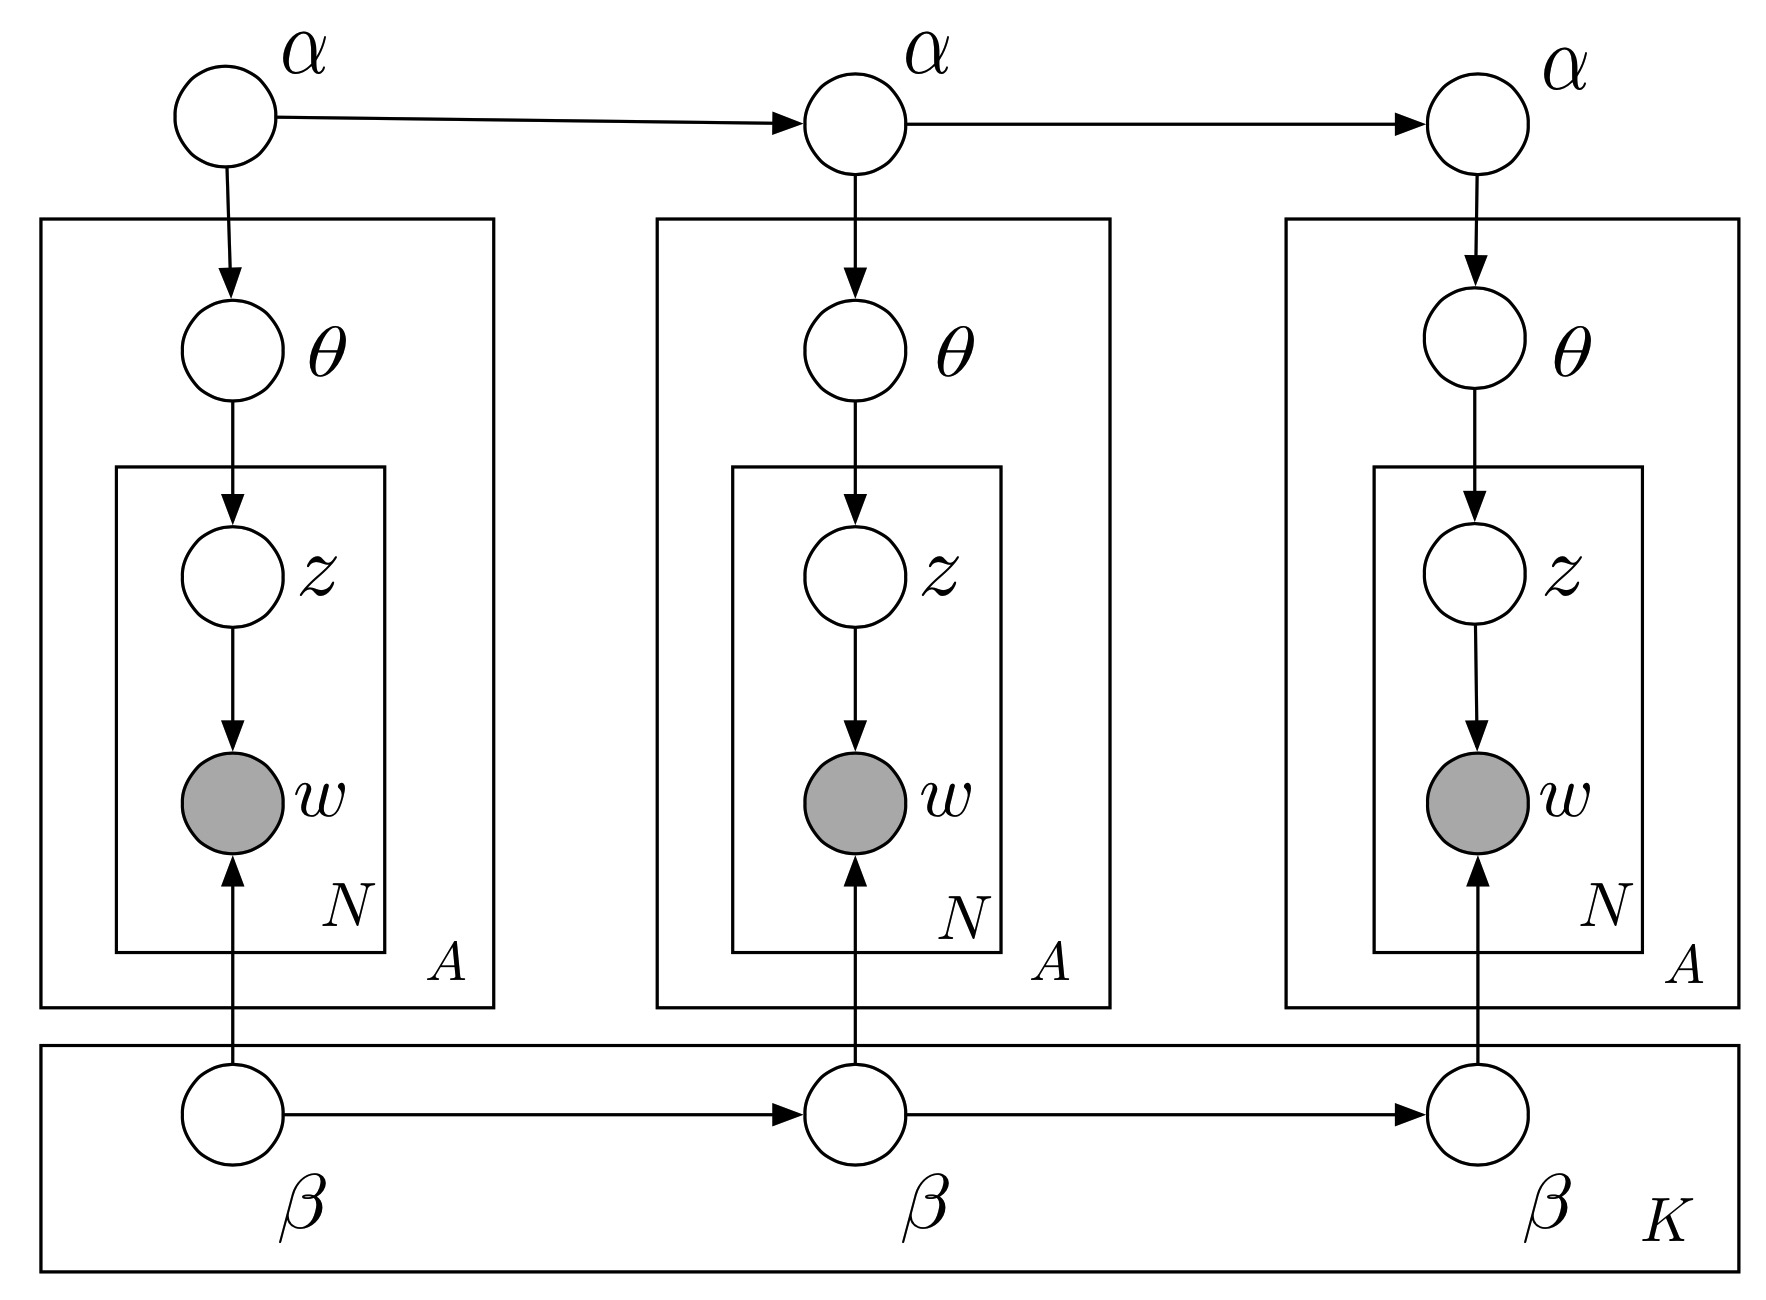
\includegraphics[width=0.6\textwidth]{dtm-graph-model}
    \caption{DTM 图模型}
    \label{fig:dtm-graph-model}
\end{figure}


在动态主题模型中,文档集按时间顺序被分割成$t$个切片,每个切片内的子文档集都用主题模型建模。切片$t$内的主题~词汇分布$\beta_t$是由$t-1$切片内的主题~词汇分布$\beta_{t-1}$演化而来的,$\beta_{t,k}$表示切片$t$内主题$k$对应的主题~词汇分布。本文作者假定状态空间中的$\beta_{t,k}$是通过链式高斯分布(Chaining Gaussian Distributions)进化的,数学公式表达见 (\ref{eq:guass})。
\begin{equation}
\label{eq:guass}
\beta_{t,k} \mid \beta_{t-1,k} \sim N \left( \beta_{t-1,k}, \sigma^2 I \right)
\end{equation}
在LDA模型中,文档~主题分布$\theta$是通过Dirichlet分布求得的。在动态主题模型中,作者用$\alpha$均值的逻辑正态(Logistic Normal with Mean $\alpha$)来表达$\theta$分布中的不确定性,切片之间$\alpha$的进化同样假定满足链式高斯分布,数学公式表达见 (\ref{eq:logistic})。
\begin{equation}
\label{eq:logistic}
\alpha_t \mid \alpha_{t-1} \sim N \left( \alpha_{t-1}, \delta ^2 I \right)
\end{equation}
出于模型的复杂性考虑,作者没有在动态主题模型中考虑主题之间的关联关系,但是作者在他的另一篇文章\cite{lafferty2005correlated}中考虑了该问题。参数评估时由于后验分布无法直接求解,所以论文中采用了两种变分方法来近似推导,分别是变分卡尔曼滤波和变分小波回归分析。

\section{文本可视化}
文本是我们获取信息的主要来源之一,然而随着互联网技术的发展,我们可访问到的文本文档以及由我们自己创造的文本信息已经远远超过了人类可阅读的极限,因此如何让人们更快,更全面地从文本文档中了解到需要的信息,成为了一个重要的研究课题。文本可视化是通过对文本信息的挖掘和分析,提取有效信息,并通过可视化技术将这些信息以图形化的方式表达出来,同时向读者提供可交互的方式来获取信息。视觉感知作为人们获取信息最直接的方式,能够使人们以更有效的方式获取大规模文本中所蕴含的关键信息。文本可视化涵盖了信息收集,数据预处理,知识表示,视觉呈现和交互设计等多个步骤(如图 \ref{fig:visual-framework})。其中数据预处理和知识表示过程,需要用到自然语言处理和数据挖掘等相关领域的知识。
\begin{figure}[htb]
    \centering%
    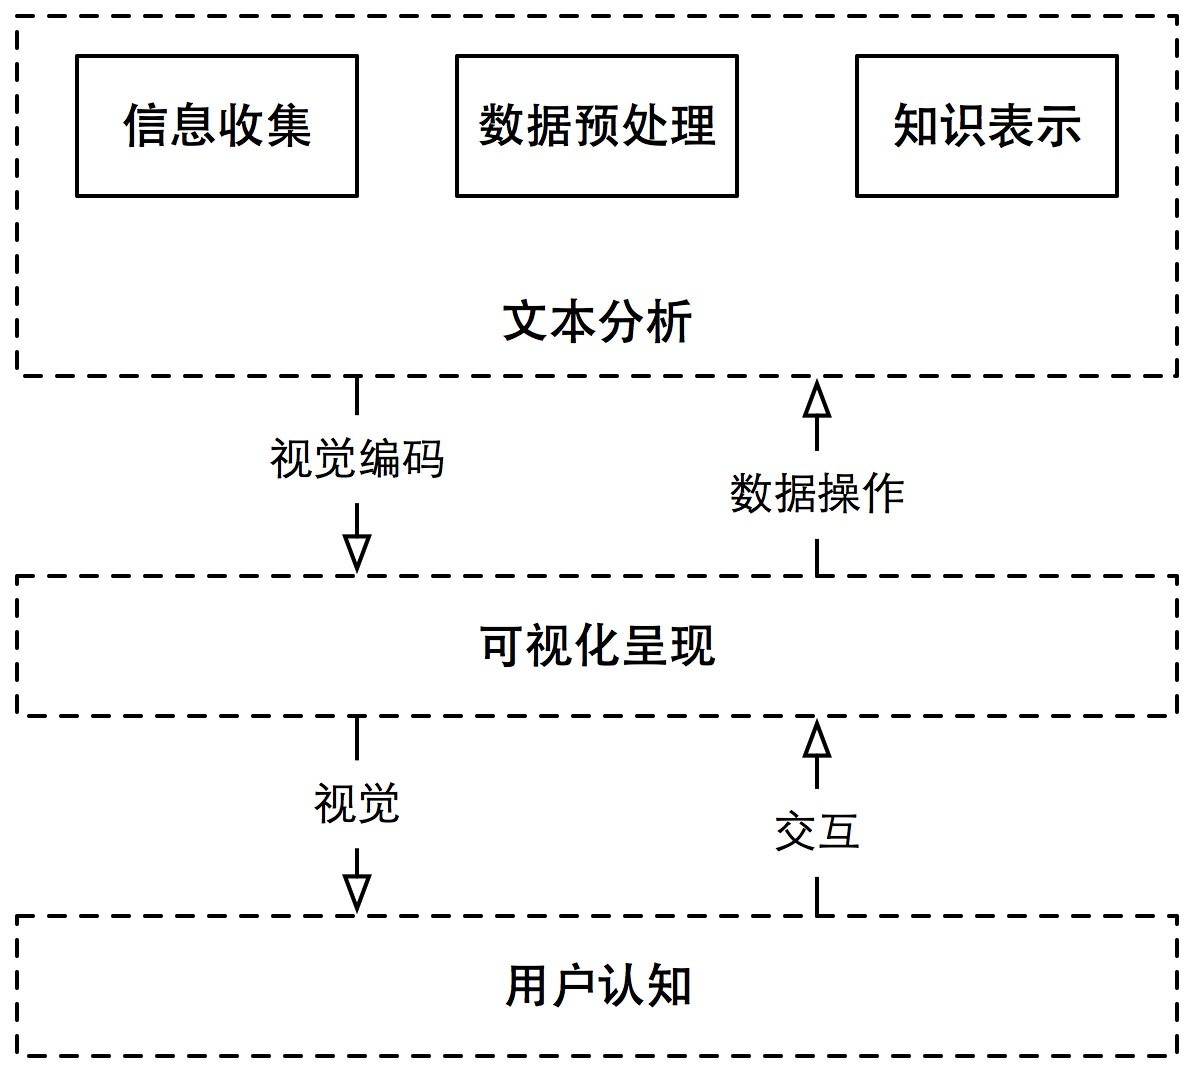
\includegraphics[width=0.6\textwidth]{visual-framework}
    \caption{文本可视化基本框架}
    \label{fig:visual-framework}
\end{figure}
本小节将介绍几种常用的文本可视化方法。

\subsection{单文本内容可视化}
标签云(Tag Cloud)又称为单词云(Word Cloud)是一种常用的文本数据可视化表现方法之一。标签通常是单个单词,标签的颜色和字体大小用于表现该标签的重要性。通过标签云可以让读者一目了然的了解到文本信息中最重要的信息是什么,并且把读者的焦点引导到重要信息上面。标签云作为一项成熟的文本可视化技术,已有了不少开源的项目(如:IBM Word-Cloud Generator\footnote{http://web.archive.org/web/20110719002236/http://www.alphaworks.ibm.com/tech/wordcloud},Wordle\footnote{http://www.wordle.net/}等)帮助用户生成各式各样的标签云,图 \ref{fig:tag-cloud}列举了一些常用标签云效果:
% BEGIN == Tag Cloud Sample
\begin{figure}[htb]
    \centering
    \subfloat[]{
        \label{fig:tag-cloud-sample1}
        
\includegraphics[width=0.33\textwidth]{tag-cloud-sample1}}
    \subfloat[]{
        \label{fig:tag-cloud-sample2}
        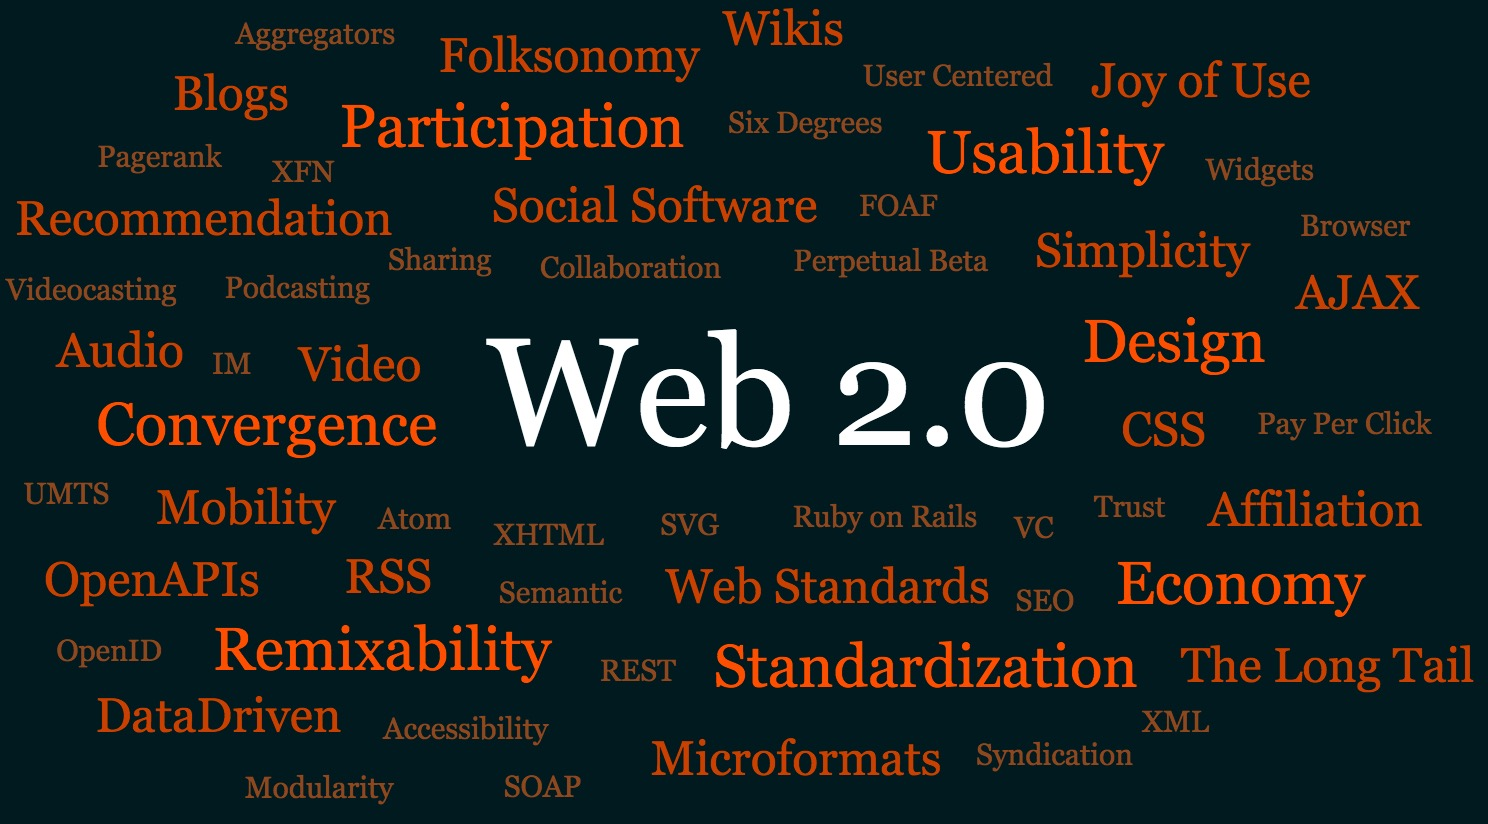
\includegraphics[width=0.33\textwidth]{tag-cloud-sample2}}
    \subfloat[]{
        \label{fig:tag-cloud-sample3}
        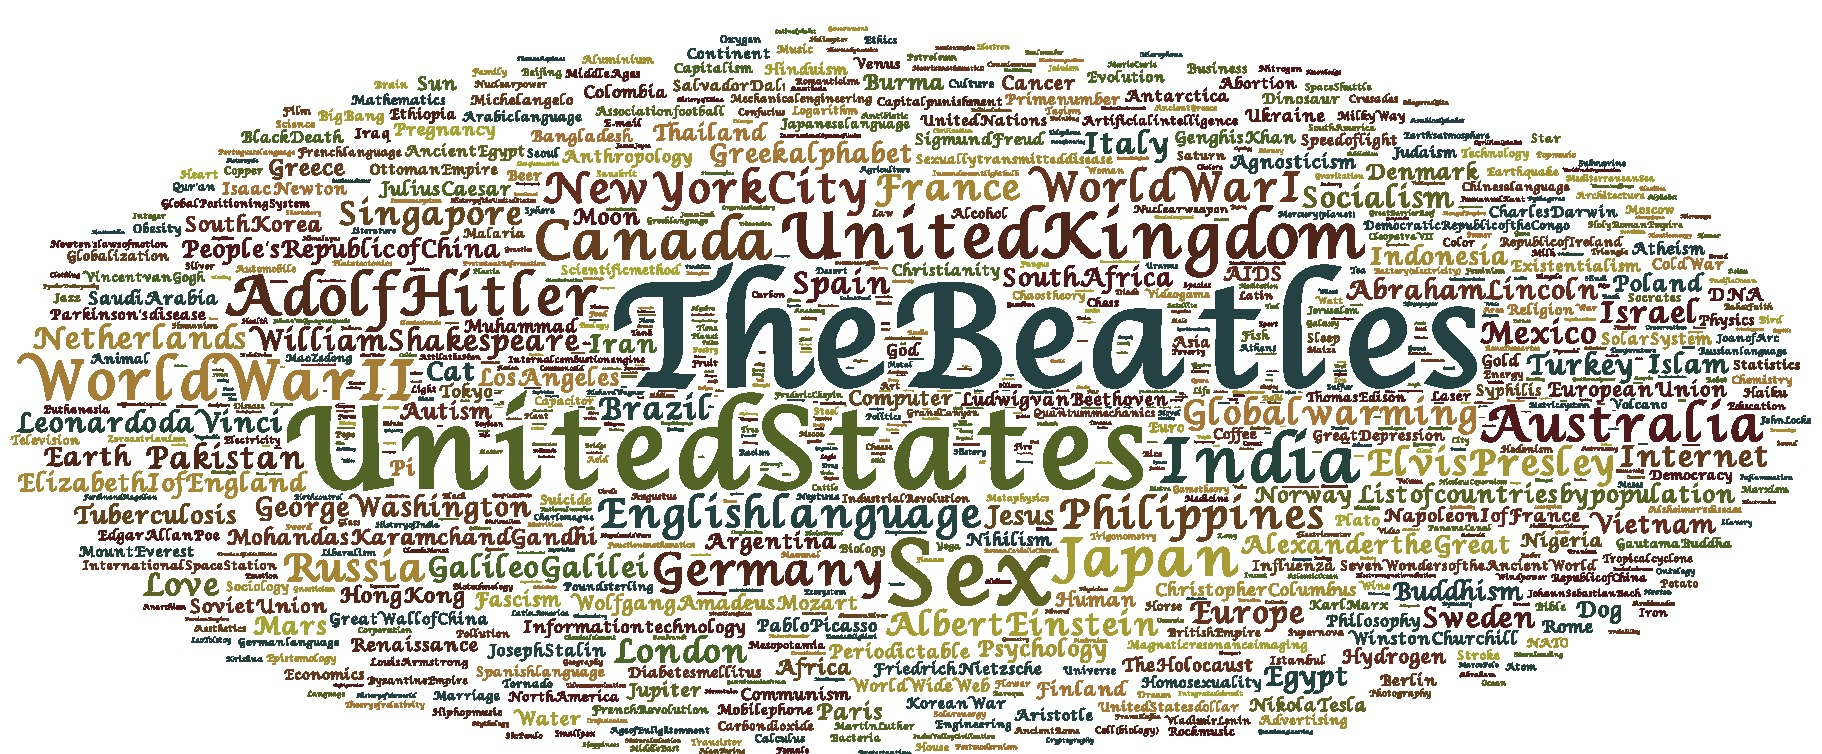
\includegraphics[width=0.33\textwidth]{tag-cloud-sample3}}
    \caption{标签云实例}
    \label{fig:tag-cloud}
\end{figure}
% END == Tag Cloud Sample

单词树(Word tree)\cite{Wattenberg2008}是针对无结构的文本数据(如:书籍,文章,演讲稿或诗歌等)的一种可视化搜索工具。通过键入关键词,单词树能够通过树状结构向你呈现所有该关键词出现的上下文信息。图形中的文字大小表示该词在文本中出现的频次,出现越频繁字体也就越大。通过搜索恰当的关键词,单词树也能很好的表现数据集的核心内容。图 \ref{fig:word-tree-sample1} 生成自科幻小说《爱丽丝梦游仙境》,根据关键词“Cried”搜索所得到的上下文信息;图 \ref{fig:word-tree-sample2} 生成自奥巴马关于战争的演讲稿,根据关键词“Iraq”搜索得到的上下文信息。 
% BEGIN == 单词树
\begin{figure}[htb]
    \centering
    \subfloat[爱丽丝梦游仙境]{
        \label{fig:word-tree-sample1}
        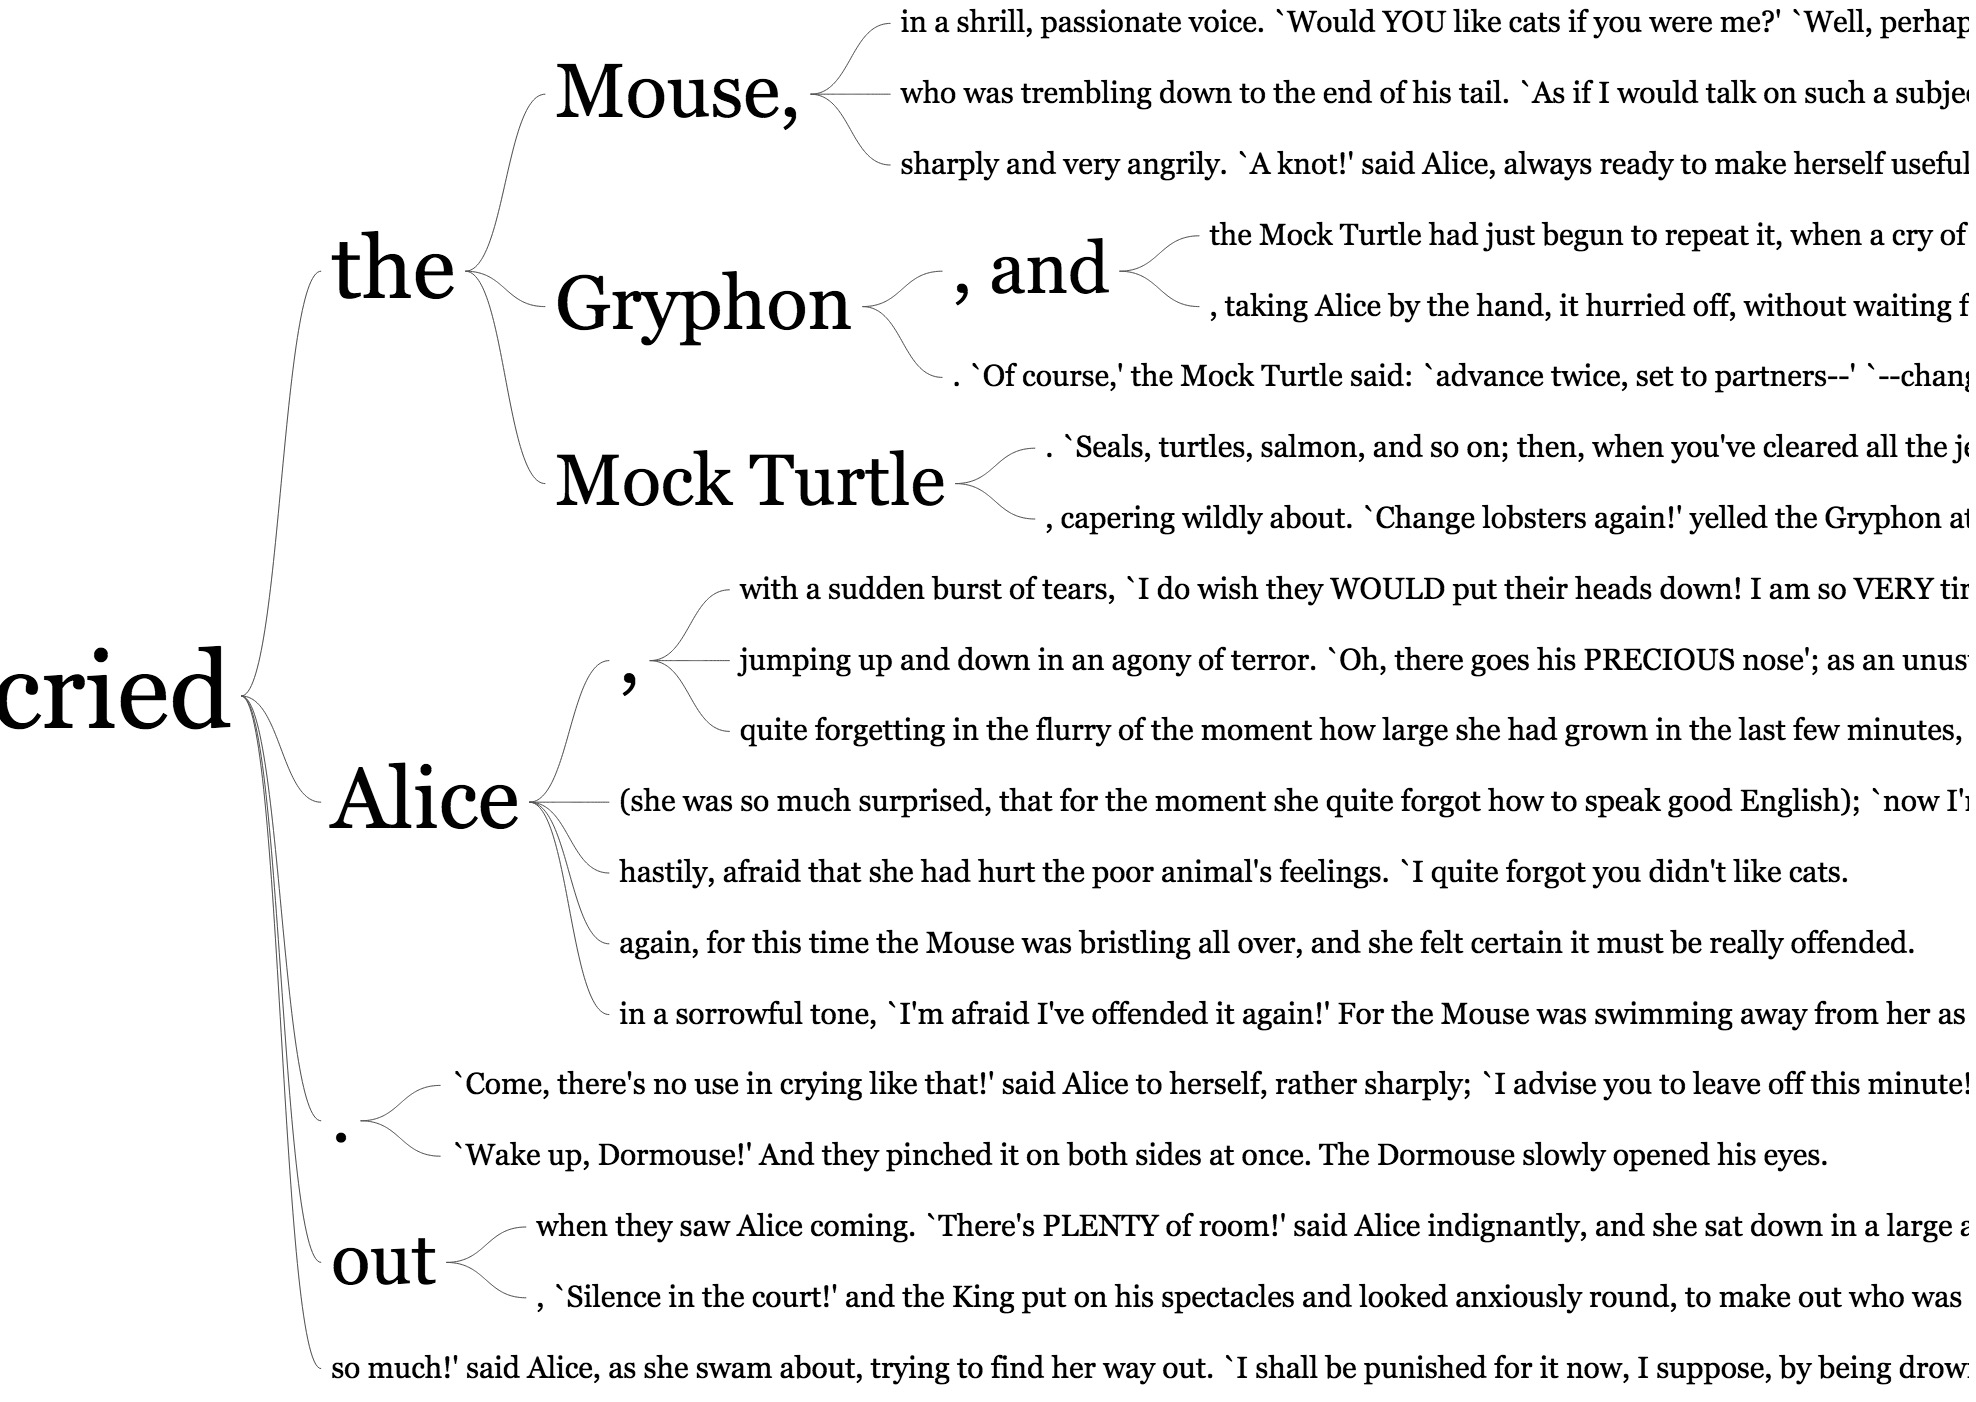
\includegraphics[width=0.465\textwidth]{word-tree-sample1}}%两个\subfloat之间没有空行
    \subfloat[奥巴马战争演讲]{
        \label{fig:word-tree-sample2}
        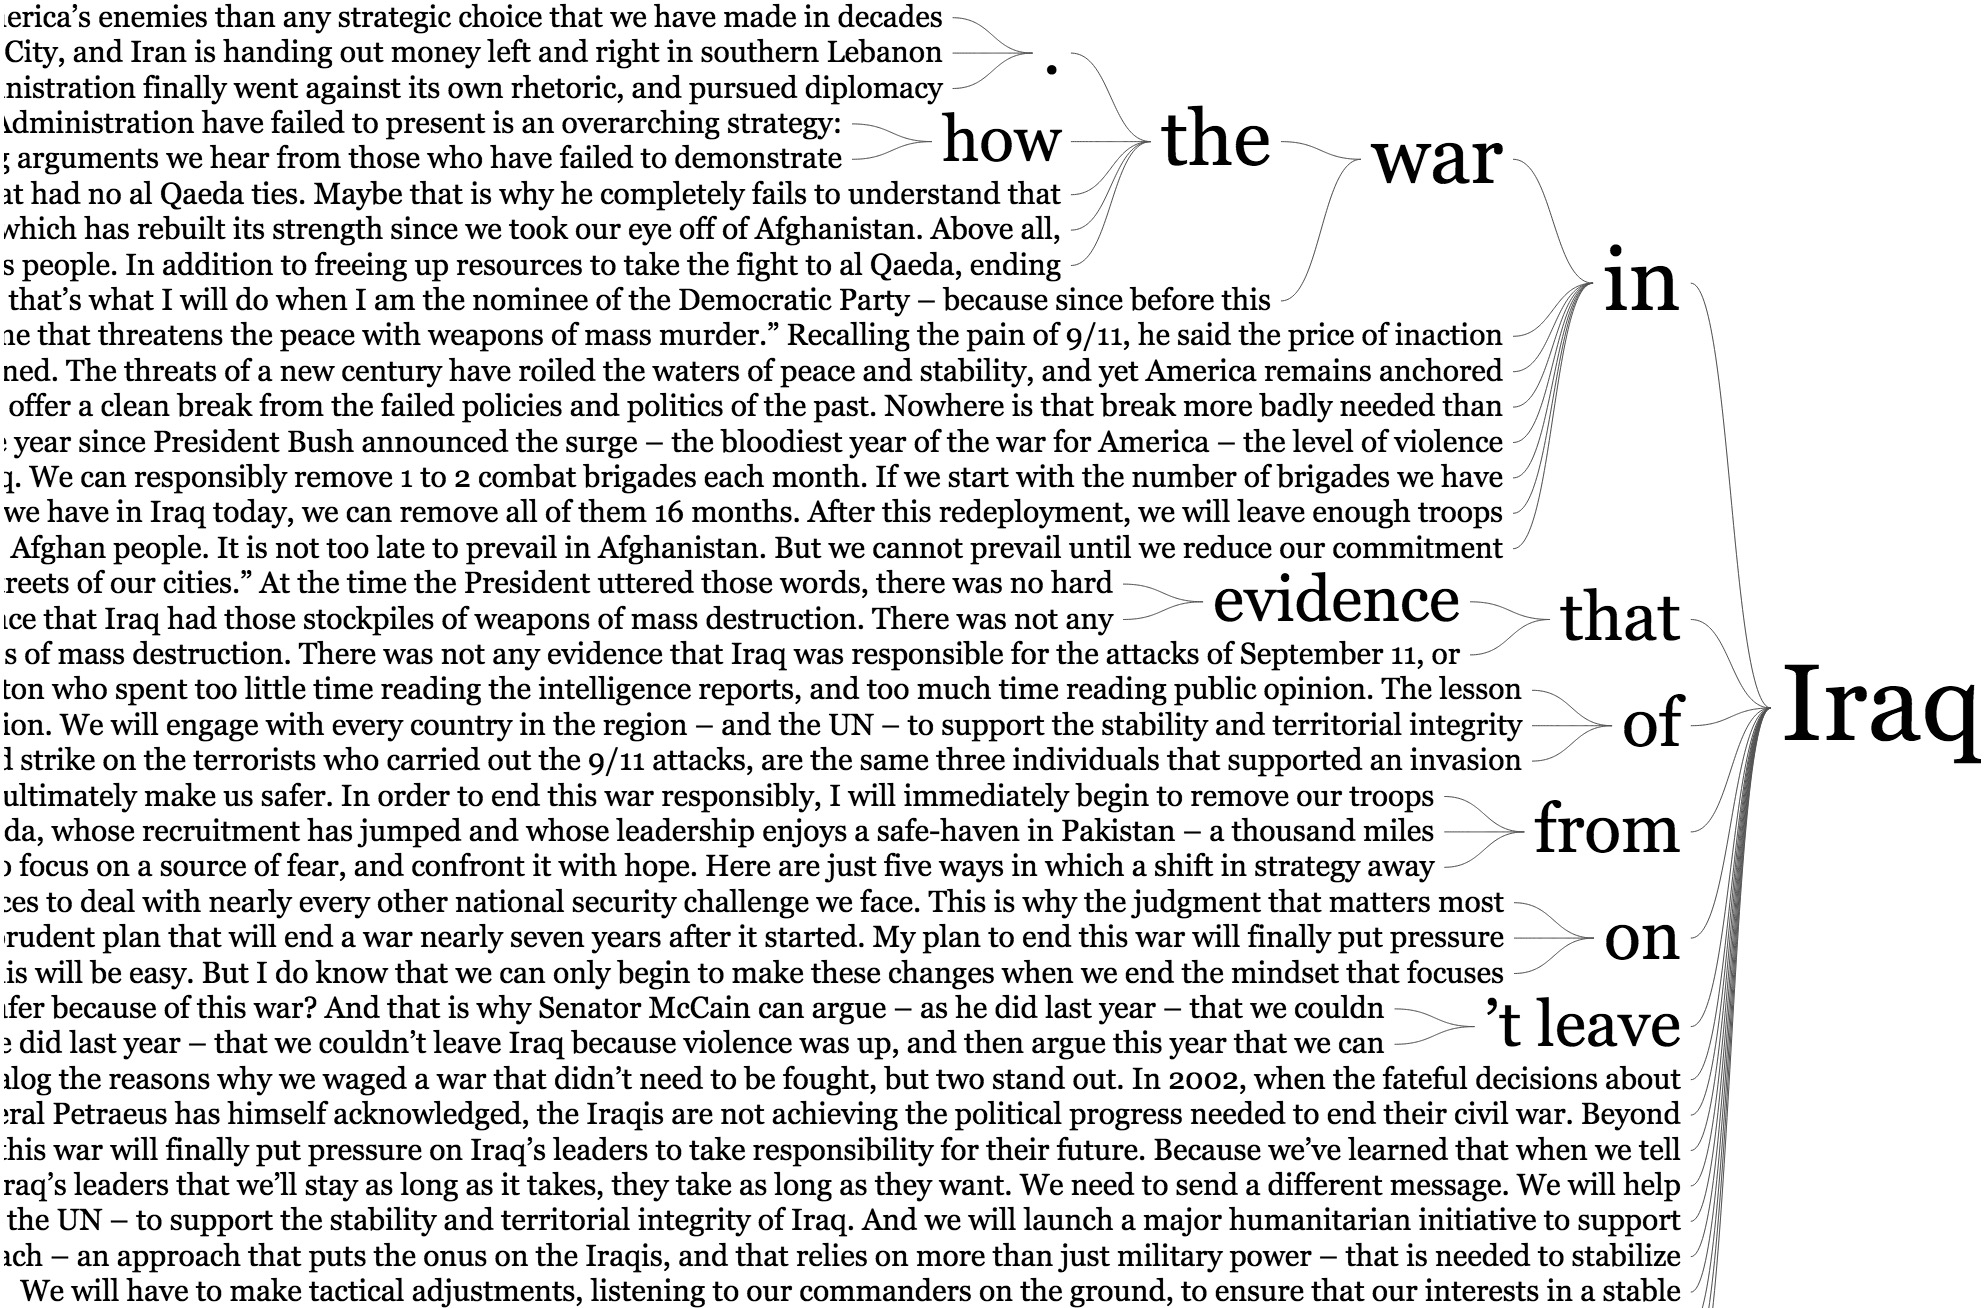
\includegraphics[width=0.5\textwidth]{word-tree-sample2}}
    \caption{单词树实例}
    \label{fig:word-tree}
\end{figure}
% END == 单词树

\subsection{多文挡可视化}
星系图(Galaxy)和主题山地(ThemeView)\cite{Wise1995} 的基本思想都是将文本信息用空间信息来表示,然后将空间信息可视化的表现出来。在Galaxy图中(如图 \ref{fig:galaxyview}),每个单独的文档都用一个灰色的点来表示,两个小灰点距离很近表示这两个文档相似度较高,相反,代表相似度低的两个文档的灰点离得就比较远。通过这种展现形式,Galaxy希望能够让读者可以很快地知道文档之间的相似关系。然而Galaxy图中,随着文档集合的变大,灰点会发生重叠和积压。ThemeView将Galaxy中的二维空间信息映射到三维空间,很好的解决了Galaxy中的灰点挤压问题。将ThemeView中的点映射到水平面上便得到了Galaxy图。在ThemeView图中(如图 \ref{fig:themescape}),每个山峰对应了一个主题,文档的主题与山峰的主题越相似,则它的高度就越高。Galaxy和ThemeView均在IN-SPIRE\footnote{http://in-spire.pnnl.gov/}软件中得以实现,该软件由Pacific Northwest National Laboratory\footnote{http://www.pnnl.gov/}设计和开发。
\begin{figure}[htb]
    \centering
    \subfloat[主题山地]{
        \label{fig:themescape}
        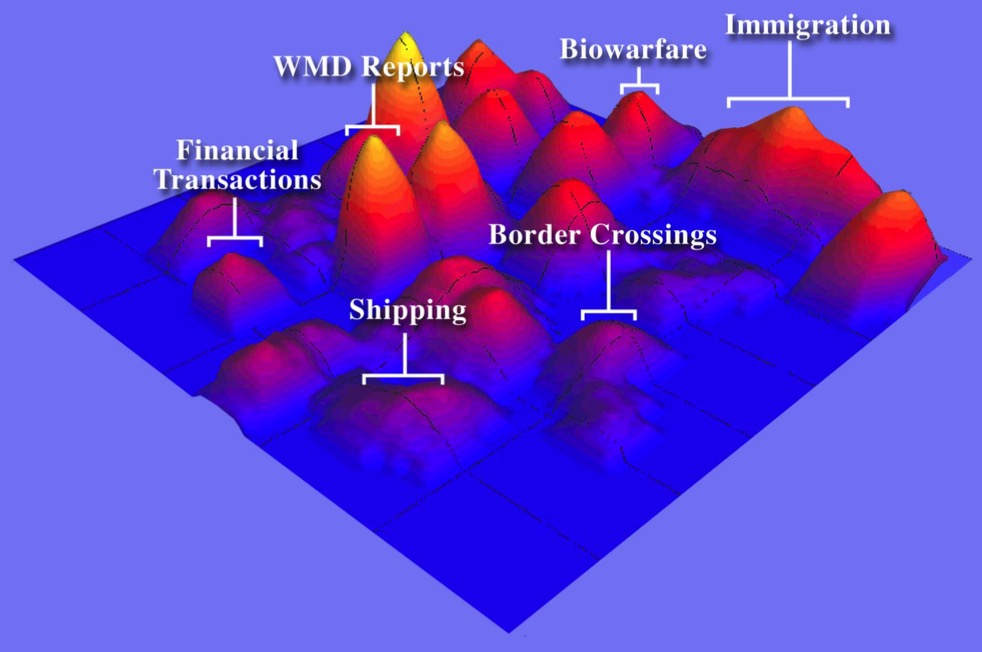
\includegraphics[width=0.305\textwidth]{themescape}}%两个\subfloat之间没有空行
    \subfloat[星系图]{
        \label{fig:galaxyview}
        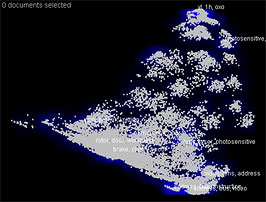
\includegraphics[width=0.265\textwidth]{galaxyview}}
    \subfloat[新闻地图]{
        \label{fig:newsmap}
        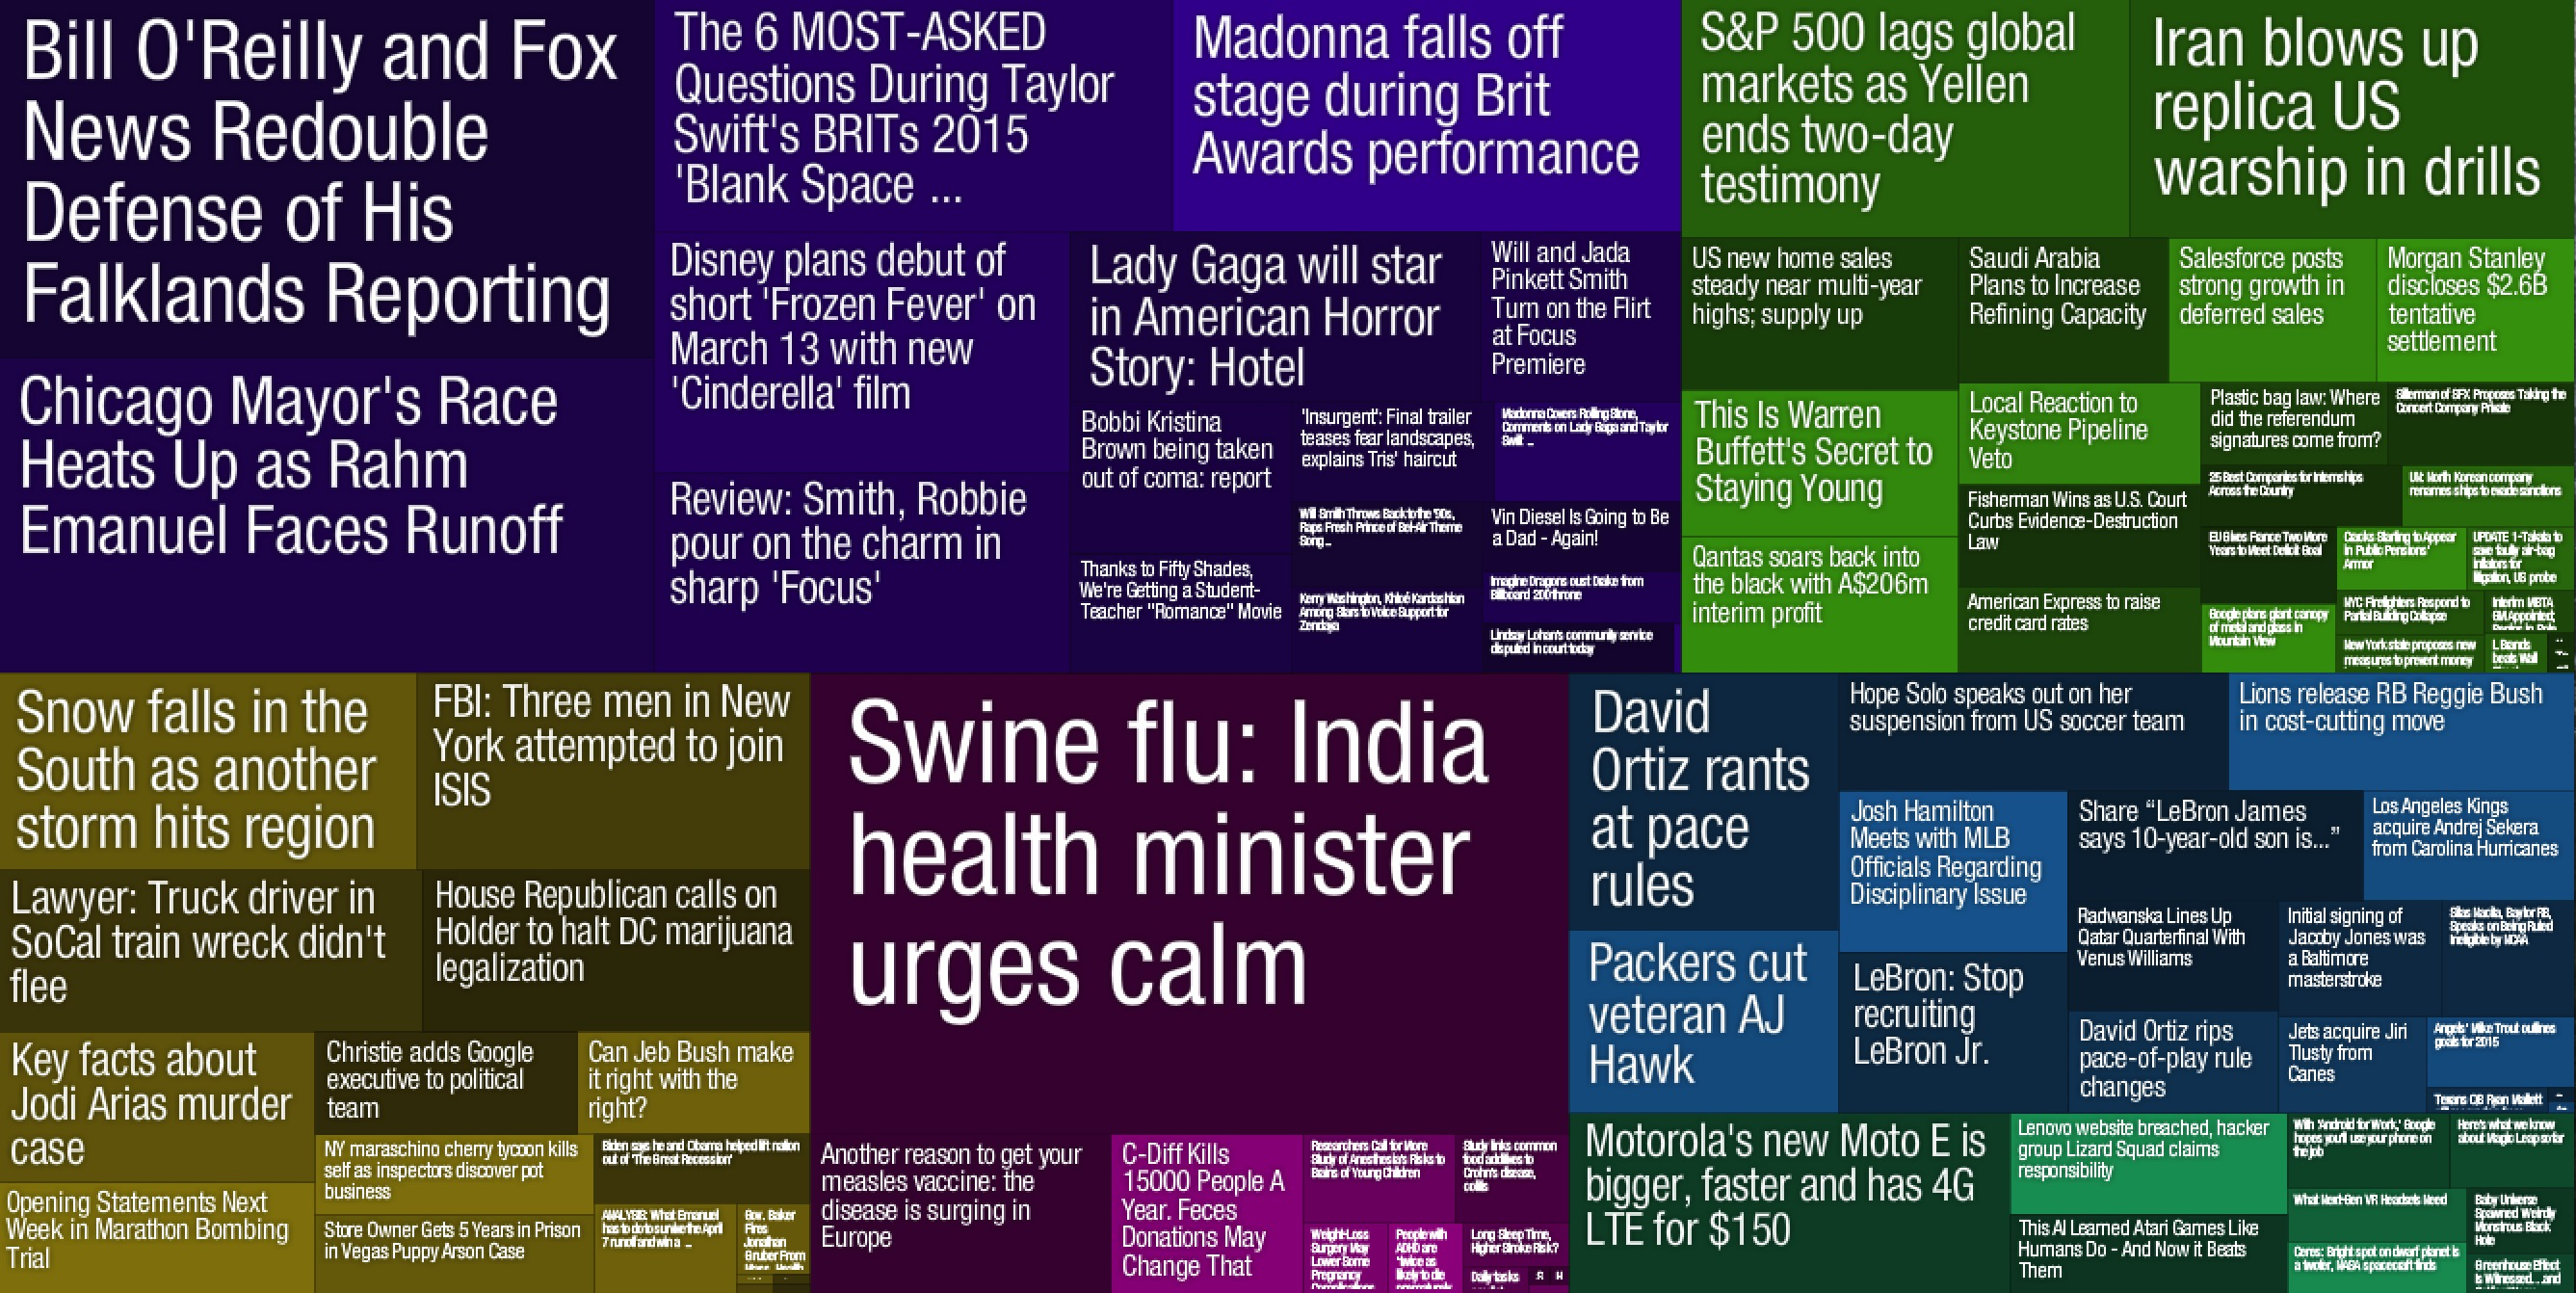
\includegraphics[width=0.4\textwidth]{newsmap}}
    \caption{多文档可视化实例}
    \label{fig:multi-doc-visual}
\end{figure}

新闻地图(Newsmap)\footnote{http://newsmap.jp/} 是一种新闻集成的方法,它可以根据新闻的受欢迎程度以及报道的数量将新闻组织在一个视觉上令人愉悦的树形图上。每个矩形方框的大小反映了新闻的热度,面积越大则该新闻故事越受欢迎,面积越小则表示该新闻故事当前还没有得到广泛的关注。同时为了使视觉上更美观,每个矩形框的着色都尽可能的与和它相邻的矩形框不一样。通过Newsmap使得读者可以很清晰的了解当前正在发生哪些新闻事件以及它们的热度(如图 \ref{fig:newsmap})。在Newsmap网站上,用户还可以根据不同的分类(如:全球,国家,商业,科技,体育,娱乐和健康)和不同的国家(如:美国,英国,法国,中国,日本等等)来过滤和展示新闻,并且你还可以自定义分类和国家,从而只保留你感兴趣的新闻内容。

\subsection{时序文本可视化}
对于时序文本,除了要呈现语料库的静态主题信息以外,更重要的是如何更好得对动态的主题变化进行可视化展现,而这也正是吸引广大研究人员的地方。下面将列举几个比较有代表性的集中方法:
% BEGIN == 时序文本可视化
\begin{figure}[htb]
    \centering
    \subfloat[主题河流]{
        \label{fig:themeriver}
        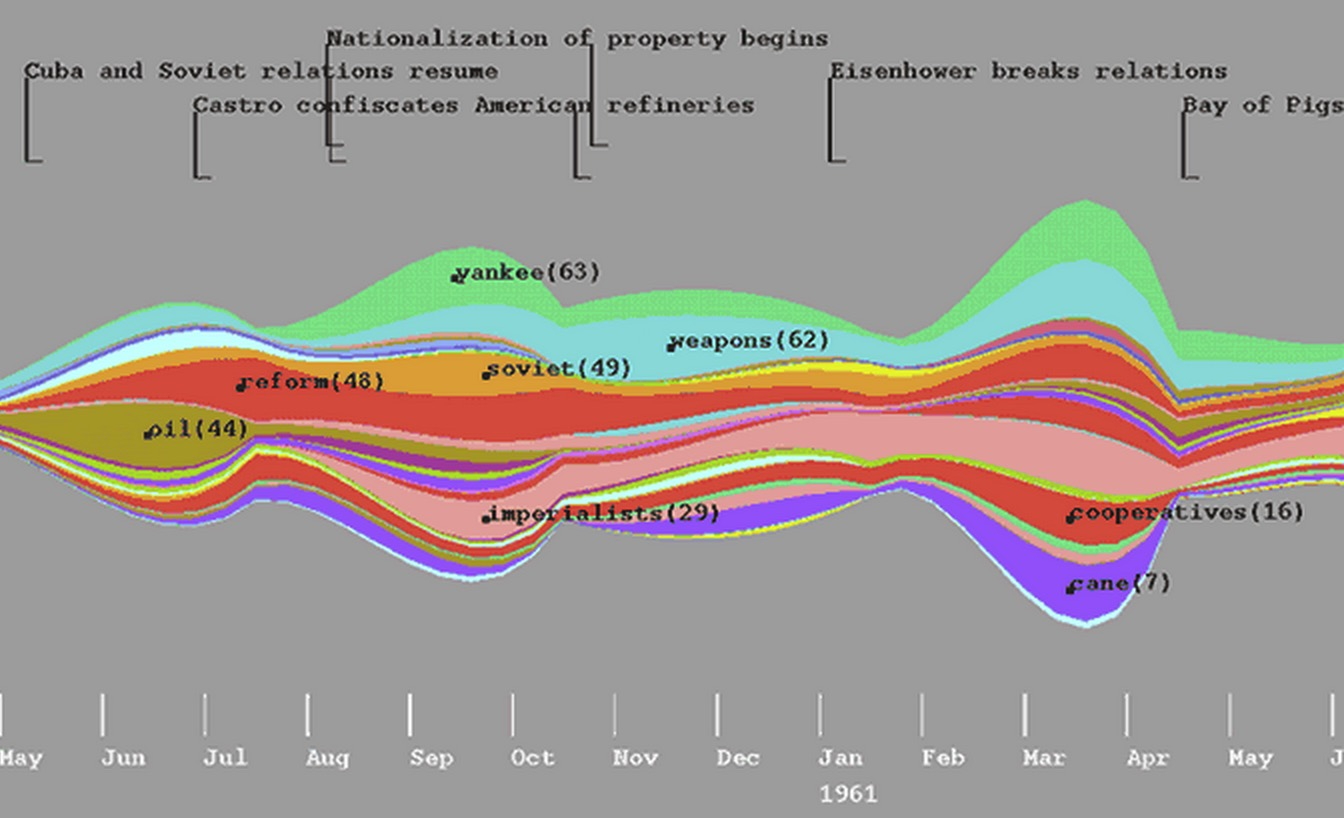
\includegraphics[width=0.45\textwidth]{themeriver}}
    \subfloat[地铁网络图]{
        \label{fig:metromap}
        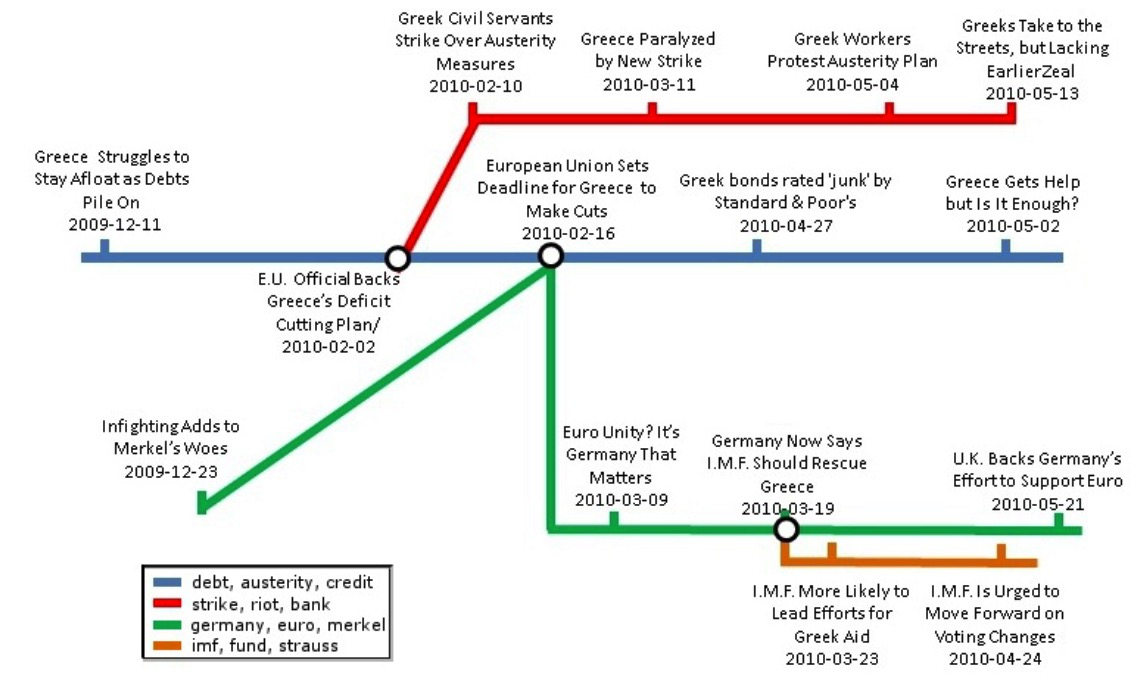
\includegraphics[width=0.45\textwidth]{metromap}}%留空行 控制换行
    
    \subfloat[文本流]{
        \label{fig:textflow}
        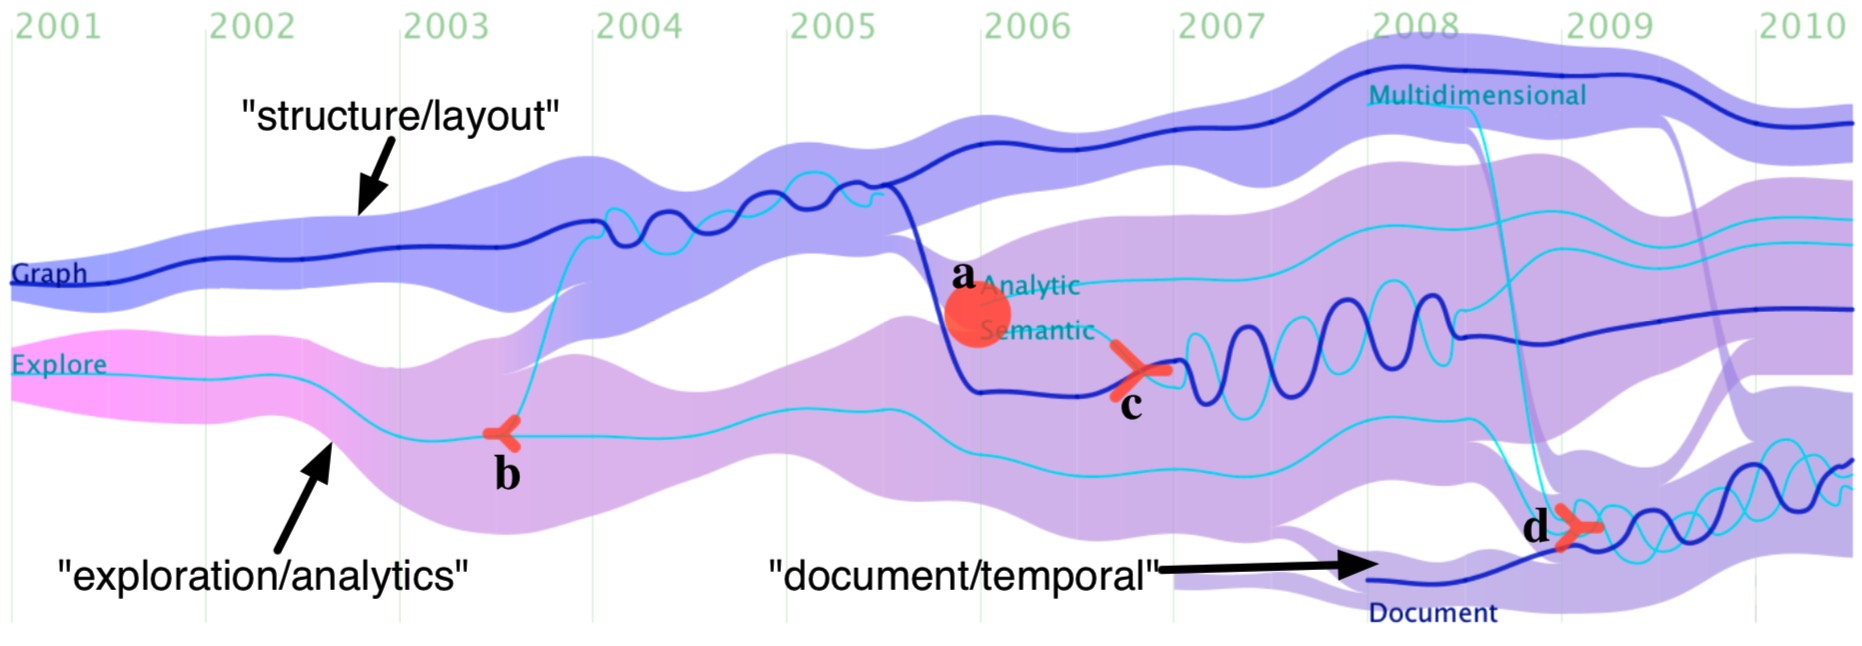
\includegraphics[width=0.9\textwidth]{textflow}}
    \caption{时序文本可视化方法举例}
    \label{fig:temporal-theme-visual}
\end{figure}
% END == 时序文本可视化

主题河流(ThemeRiver)\cite{Havre:2000}可以帮助用户辨识大规模文档集合中与时间相关的模式,趋势以及关联关系。文档集合中的主题通过沿时间轴从左往右的河流来表示。主题河流通过不同颜色的色带表示不同的主题,色带的宽度表示主题的强度,色带越宽表示该主题在该时间段内的强度越强;反之,色带越窄表示主题在该时间段的影响越小,如图 \ref{fig:themeriver}所示。

地铁网络图(Metro Map)\cite{shahaf2012trains} 的想法缘自地铁的网络图,它是由一系列代表事件线索的线条组成,每个线条代表了事件的一个方面,线条的交叉和重叠部分表示不同线索之间的关联和融合。通过 Metro Map 用户可以很快的获得一个故事的整体情况。(如图 \ref{fig:metromap}所示)

文本流(TextFlow)\cite{Weiwei:2011}是用于分析多个主题之间演化关系的文本可视化方法。生成图 \ref{fig:textflow}的数据来自2001年到2011年在VisWeek上发表的所有文章,Textflow很好的反映了主题在这段时间的演化。Textflow采用了一种流图的展现方法,每个流代表一个主题,流的宽度表示在这个时间点上与该主题相关的文档数量,数量越多,宽度越宽。区别于ThemeRiver,TextFlow还能表现关键事件,包括主题的产生,终结,分裂和合并,并分别用不同的符号表示。同时,Textflow还能将主题内关键词的联系展示出来,每个流中的线表示某个关键字,用户可以根据这三方面分析推断主题的变化,以及变化的原因。

Storyline 描述的是人物之间随时间变化的交互关系,它将这些复杂的信息在一张图形上展现出来。该方法是受 Mounroe 发布在著名漫画网站 XKCD 的 "Movie Narrative Charts" \cite{xkcd657} 的启发。在这个连载漫画中,手绘的 Storyline 用于概括电影中角色之间的互动(如图 \ref{xkcd},其中X轴表示时间,每个线条分别代表一个角色)。
%% BEGIN == XKCD 手绘图
\begin{figure}[htb]
    \centering
    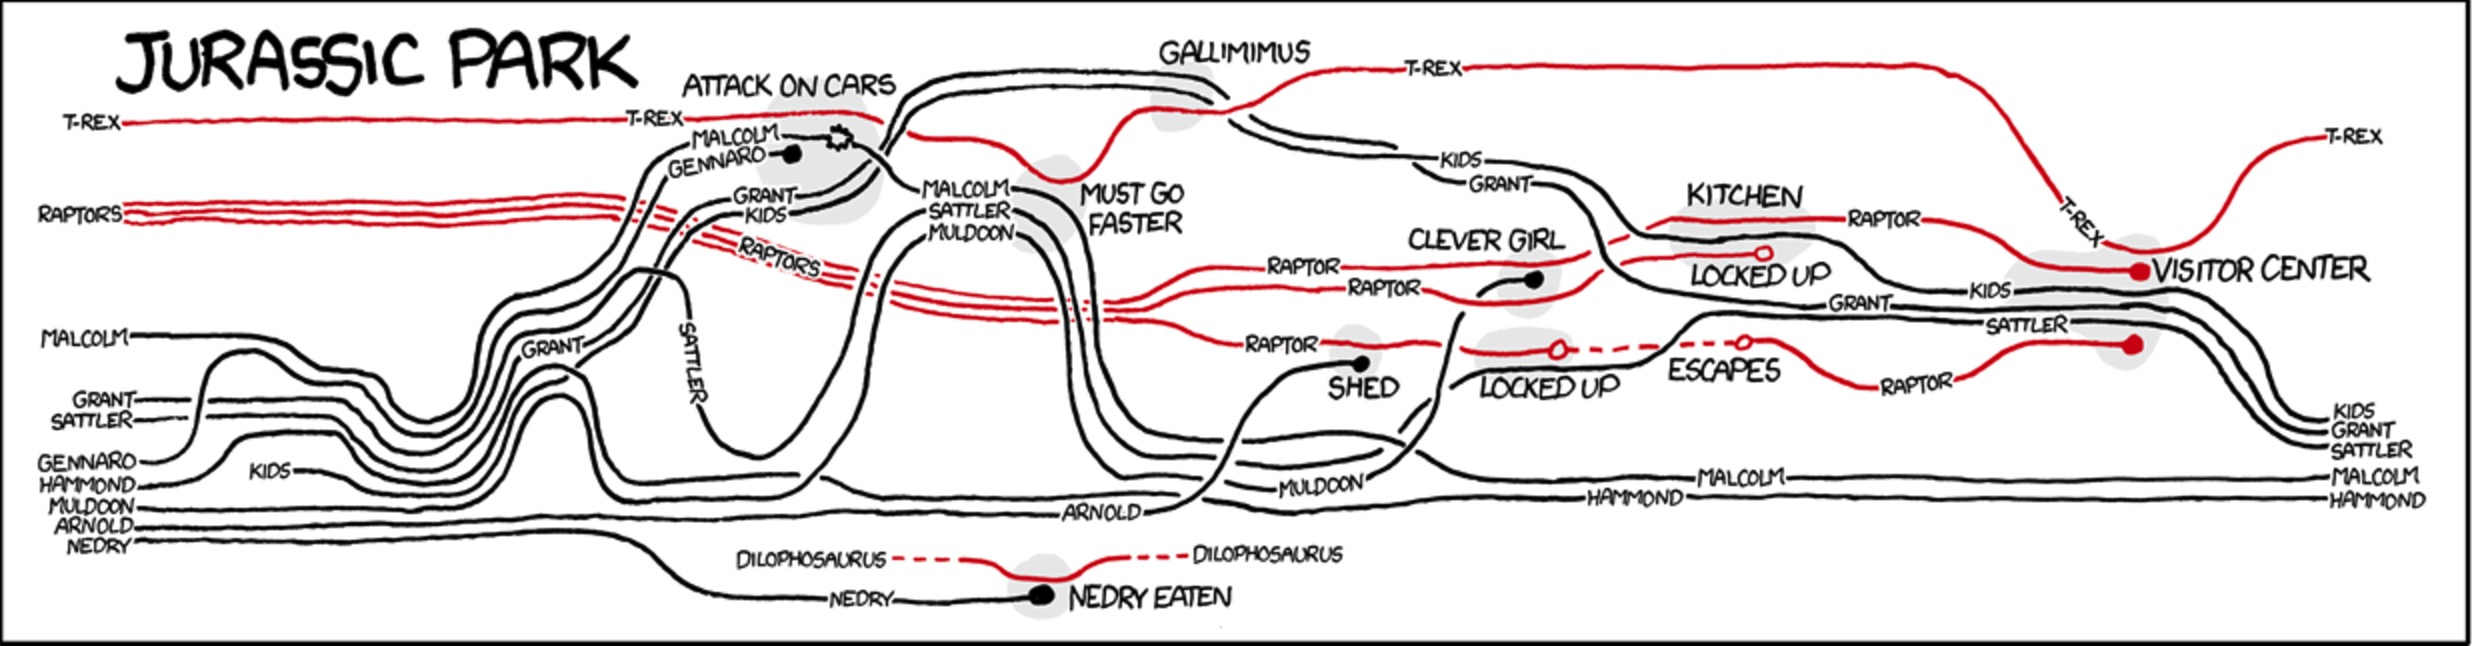
\includegraphics[width=\textwidth]{xkcd_jurassic_park}
    \caption{Jurassic park 人物关系叙事图}
    \label{xkcd}
\end{figure}
%% END == XKCD 手绘图
相比其它时间轴相关的可视化方法,Storyline 通过线条来表示故事中的实体,并且通过与实体关联的线条的之间的距离变化来表示实体之间的关联关系。

\section{本章小结}
本章主要介绍了与本课题相关的一些研究工作,为后文的研究内容提供一些基础知识,以便更好的理解。我们首先介绍了概率主题模型的基本原理和模型推导方法,并详细阐述了LDA\cite{Blei:2003}和DTM\cite{Blei:2006}两个具体的主题模型,包括它们的图模型、文档生成过程以及参数的推导方法。接着我们介绍了文本可视化的一般方法和基本框架,并分三个类别介绍了文本可视化的常用方法。针对单文档可以采用标签云和单词树,针对多文本文档集合可以采用新闻地图和主题山地等方法,针对时序文本集合可以采用主题河流、地铁网络图、文本流和Storyline。



